\documentclass[a4paper]{article}
\usepackage[a4paper, hmargin = 2cm, vmargin=3cm]{geometry}
\usepackage[T1]{fontenc}
\usepackage{natbib}
\usepackage[french]{babel}
\usepackage[utf8x]{inputenc}
\usepackage{amsmath}
\usepackage{graphicx}
\usepackage{wrapfig}
\usepackage{caption}
\usepackage{float}
\usepackage[colorinlistoftodos]{todonotes}
\usepackage{url}
\usepackage{bm}
\usepackage[backref=page]{hyperref}
\usepackage{soul}
\usepackage{longtable,booktabs}
\usepackage{listings}
\usepackage{mathtools}
\usepackage{textgreek}
\usepackage{svg}
\usepackage{subcaption}
\usepackage{acronym}
\usepackage[automake]{glossaries}  % handle acronyms and glossary
\usepackage[numbib,nottoc]{tocbibind}
\usepackage{fancyhdr}
% \usepackage[printwatermark]{xwatermark}
\usepackage{xcolor}
\usepackage{etoolbox}
\usepackage{textcomp}
\usepackage{gensymb}
\usepackage{cleveref}
\makeatletter
\patchcmd{\BR@backref}{\newblock}{\newblock(page~}{}{}
\patchcmd{\BR@backref}{\par}{)\par}{}{}
\makeatother
\hypersetup{
    colorlinks,                   % use colored links
    linkcolor=[rgb]{0,0.31,0.55},   % toc, fig, eq, table
    citecolor=[rgb]{0.3,0.3,0.3},  % citation and references 
    urlcolor={blue!60!black}     % url
}

% \newwatermark[allpages,color=red!10,angle=60,scale=4.4,xpos=-20,ypos=10]{CONFIDENTIEL}

\newenvironment{changemargin}[2]{%
\begin{list}{}{%
\setlength{\topsep}{0pt}%
\setlength{\leftmargin}{#1}%
\setlength{\rightmargin}{#2}%
\setlength{\listparindent}{\parindent}%
\setlength{\itemindent}{\parindent}%
\setlength{\parsep}{\parskip}%
}%
\item[]}{\end{list}}

\makeglossaries

\newglossaryentry{apprentissage}
{
  name=Apprentissage informatique,
  text=apprentissage informatique,
  description={Branche de l'intelligence artificielle voulant donner à l'ordinateur la capacité de s'améliorer dans la résolution d'un problème}
}

\newglossaryentry{surapprentissage}
{
    name=Surapprentissage,
    text=surapprentissage,
    description={Le réseau n'est capable de répondre qu'aux données identiques à l'entraînement et ne se généralise pas. 
    Un réseau entraîné sur trop d'époques pour trop peu de données en est souvent la cause}
}
\newglossaryentry{echantillon}
{
    name=\'{E}chantillon,
    text=\'{e}chantillon,
    description={Valeur du signal à un temps donné.
    Il est situé entre -1 et 1}
}
\newglossaryentry{signal}
{
    name=Signal,
    text=signal,
    plural=signaux,
    description={Représentation d'un son sous la forme de variations de valeurs en fonctions du temps}
}
\newglossaryentry{fourier}
{
    name=Transform\'{e}e de Fourier,
    text=transform\'{e} de Fourier,
    description={Calcul permettant d'obtenir les fréquences présentes dans un signal}
}

\newglossaryentry{sequenceur}
{
	name=S\'{e}quenceur,
	text=s\'{e}quenceur,
	description={Logiciel permettant le travail de l'audio pour l'enregistrement, le mixage, ou encore la création}
}

\newglossaryentry{latence}
{
	name=Latence,
	text=latence,
	description={Phénomène apparaissant si le temps de calcul d'un échantillon est plus grand que le temps maximum disponible pour ce calcul}
}

\newglossaryentry{plugin}
{
	name=Plugin,
	text=plugin,
	description={Module d'extension apportant des fonctionnalités à un logiciel}
}

\DeclarePairedDelimiter{\ceil}{\lceil}{\rceil}
\pagestyle{fancy}
\fancyhf{}
\lhead{Maxence Lévêque}
\rhead{Simulation d'un amplificateur de guitare 
  à l'aide d'un réseau de neurones}
\rfoot{\thepage}
\lfoot{\leftmark}

\begin{document}

\def\labelitemi{--}

\begin{titlepage}

  \newcommand{\HRule}{\rule{\linewidth}{0.5mm}} % Defines a new command for the horizontal lines, change thickness here
  \center    
  %----------------------------------------------------------------------------------------
  %	HEADING SECTIONS
  %----------------------------------------------------------------------------------------
  
  \textsc{\LARGE Université de Bordeaux}\\[0.5cm]
  \textsc{\LARGE -}\\[0.5cm]
  \textsc{\Large Orosys - Two notes Audio Engineering}\\[0.5cm]
  \textsc{\large Rapport de stage}\\[1cm]
  
  %----------------------------------------------------------------------------------------
  %	TITLE SECTION
  %----------------------------------------------------------------------------------------
  
  \HRule \\[0.4cm]
  { \huge \bfseries Simulation d'un amplificateur de guitare 
  à l'aide d'un réseau de neurones}\\[0.4cm]
  \HRule \\[2cm]
   
  %----------------------------------------------------------------------------------------
  %	AUTHOR SECTION
  %----------------------------------------------------------------------------------------
  
  \begin{minipage}{0.4\textwidth}
  \begin{flushleft} \large
  \emph{Auteur:}\\
  Maxence \textsc{Lévêque}
  \end{flushleft}
  \end{minipage}
  ~
  \begin{minipage}{0.4\textwidth}
  \begin{flushright} \large
  \emph{Maître de stage:} \\
  Yann \textsc{Bayle}\\[1cm]

  \emph{Tuteur de stage:}\\
  Pierre \textsc{Hanna}\\

  \end{flushright}
  \end{minipage}\\[2cm]

    
  %----------------------------------------------------------------------------------------
  %	LOGO SECTION
  %----------------------------------------------------------------------------------------
  
  \begin{minipage}{0.49\textwidth}
    \begin{flushleft}
      \large
    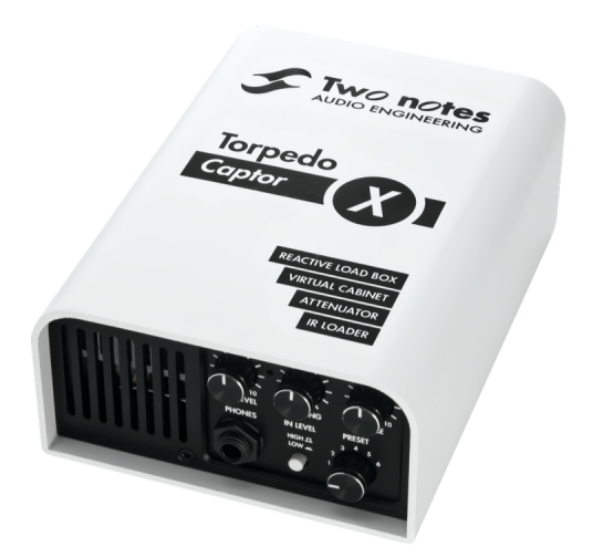
\includegraphics[width=0.5\linewidth]{../img/captorx}\\ % logo univ
  \end{flushleft}
    
    \end{minipage}
    ~
    \begin{minipage}{0.49\textwidth}
    \begin{flushright} \large
      
\includegraphics[width=0.5\linewidth]{../img/logo_orosys}\\[1cm]
      
\includegraphics[width=0.5\linewidth]{../img/logo_twonotes}\\[1cm]
    \end{flushright}
    \end{minipage}\\[2cm]
    \begin{center}
      {\huge \textsc{Document Confidentiel} \\[2cm] }
    \end{center}

   
  %----------------------------------------------------------------------------------------
  %----------------------------------------------------------------------------------------
  %	DATE SECTION
  %----------------------------------------------------------------------------------------
  \vspace*{\fill}
\begin{center}
{\large Mars-Août 2020 \\ }
\end{center}
  
\end{titlepage}

%------------------------------
%-     END OF TITLE PAGE      -
%------------------------------
\newpage
\section*{Summary}

English summary.

\newpage
\section*{Avant-propos}

Avant-propos optionnel.

\newpage
\section*{Remerciements}

Remerciements

\newpage
\begingroup
\hypersetup{linkcolor={white!0!black}}
\thispagestyle{empty}
\tableofcontents
\thispagestyle{empty}
\endgroup

\newpage
\section{Introduction}
\subsection{Présentation d'Orosys}

La société Orosys avec sa marque \textit{Two notes Audio Engineering}\footnote{\url{https://www.two-notes.com/}} conçoit des outils pour la prise de son silencieuse d’amplificateurs de guitares et basses.
Elle produit du matériel comme des atténuateurs de puissance permettant de baisser le volume d'une enceinte sans baisser la puissance de l'amplificateur.
La \autoref{img:captorX} présente le Captor X, atténuateur de puissance et simulateur d'enceinte.
Orosys fait également des préamplificateurs qui permettent d'apporter des modifications au son d'entrée de l'amplificateur avec par exemple Le Lead présenté à la \autoref{img:leLead}.
Elle propose des logiciels permettant la reconstitution de l’enceinte, du microphone et de la salle d’enregistrement avec le Torpedo Wall Of Sound.
Orosys aimerait étendre sa gamme de produits à l’émulation d’amplificateurs.
De nos jours, de nombreuses marques s’imposent comme les leaders de ce combat technologique en proposant des simulations d'amplificateurs connus avec une plus ou moins grande fiabilité.
Par cela, on entend une restitution de la signature sonore perceptuellement proche de l’outil réel utilisé dans les mêmes conditions.
C’est une tâche complexes qui rencontre de multiples obstacles tels que la scepticité des consommateurs et la difficulté technique de la tâche.

Exemple de double figure.

\begin{figure}[H]
  \centering
  \begin{subfigure}{.49\textwidth}
    \centering
    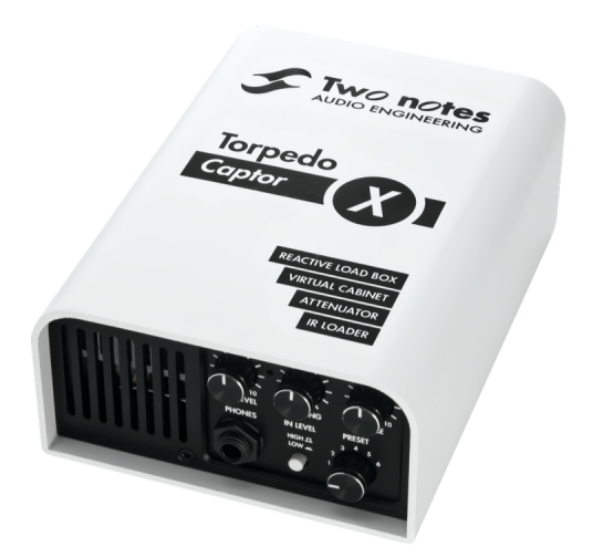
\includegraphics[width=\linewidth, height=5cm, keepaspectratio]{../img/captorx}
     \caption{L'atténuateur de puissance Torpedo Captor X}
    \label{img:captorX}
  \end{subfigure}
  \begin{subfigure}{.49\textwidth}
    \centering
    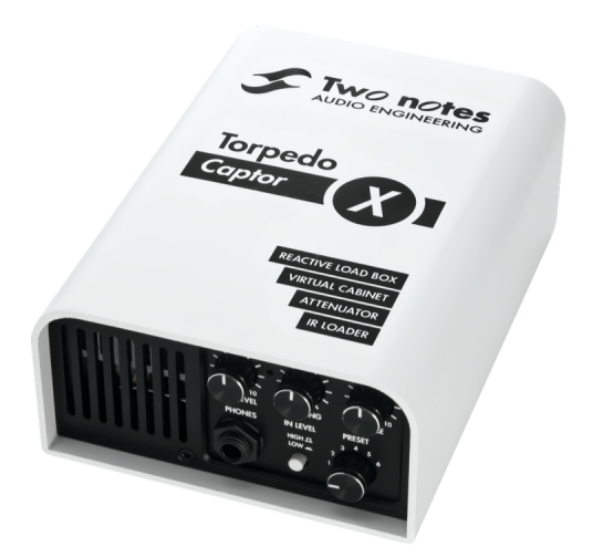
\includegraphics[width=\linewidth, height=5cm, keepaspectratio]{../img/captorx}
     \caption{Le préamplificateur Le Lead}
    \label{img:leLead}
  \end{subfigure}
  \caption{Produits commercialisés par Two notes Audio Engineering}
  \label{img:produits_twonotes}
\end{figure}

Exemple de citation de la \autoref{img:produits_twonotes}.

\subsection{Contexte et enjeux}

Exemple de glossaire avec le mot \gls{signal}.
Au singulier \glspl{echantillon} et maintenant avec du pluriel \glspl{echantillon}.

Mot en \textit{italique}.

Passage forcé à la ligne.\\
Visible ici.

\subsubsection{Sous-sous section}

\par Nouveau paragraphe.

Liste
\begin{itemize}
  \item Item 1
  \item Item 2
\end{itemize}

Liste numérotée
\begin{enumerate}
  \item Item 1
  \item Item 2
\end{enumerate}

On sait que A donne B quand on a C \citep{cho2014}.

\cite{cho2014} ont montré que D implique E.

Exemple de citation d'un article de journal par \cite{Schmitz2019}, d'un livre par \cite{Bracewell1986} et d'un article de conférence par \cite{Wright2019}.

Exemple d'acronyme \ac{LSTM} utilisé pour la première fois dans le texte.
Exemple d'acronyme \ac{LSTM} utilisé pour la deuxième fois dans le texte.

On va forcer une nouvelle page.

\newpage

Comme ceci.

On peut aussi référencer des sections en disant qu'on le verra dans la \autoref{sec:referenced}.

\section{Section référencée}
\label{sec:referenced}

Exemple de nombre $ 8,4*10 ^{6} $ intégré dans le texte.

L'\autoref{eq:nrmse} montre que A donne B.
\begin{equation}
NRMSE = \sqrt{\dfrac{\sum_{k=0}^{K}(y[k] - \hat{y}[k])^{2}}{\sum_{k=0}^{K}y[k]^{2}}}
\label{eq:nrmse}
\end{equation}

Pour 80\% et pour R\&D il faut mettre un escape char.

Utilisation de math dans le texte tel que \textmu.

Le \autoref{table:res_networks_test} montre un exemple de tableau.

\begin{table}[!h]
    \centering
    \begin{tabular}{c|ccc|ccc}
        Réseau   &       MSE        &      ESR      &   CC         & MSEa    & ESRa     & CCa\\
        \hline
        GRU    & $ 4,24e10^{-6} $ &  $ 458,81  $  & $ 76,6\%  $  & $0,001$ & $ 0,54 $ & $ 78,9\% $\\
        ConvGRU    & $ 7,93e10^{-7} $ &  $ 85,70  $  & $ 83,9\%  $  & $8,24e10^{-4}$ & $ 0,22 $ & $ 88,1\% $\\
        2LSTM    & $ 3,49e10^{-6} $ &  $ 377,19  $  & $ 84,2\%  $  & $0,0016$ & $ 0,28 $ & $ 87,4\% $\\
        2Conv1LSTM    & \bm{$ 6,48e10^{-6} $} &  \bm{$ 19,45  $}  & \bm{$ 98,7\%}  $  & \bm{$6,49e10^{-5}$} & \bm{$ 0,013 $} & \bm{$ 99,3\% $}\\
    \end{tabular}
    \caption{Résultats obtenus avec les réseaux testés}
    \label{table:res_networks_test}
\end{table}

\newpage

\bibliographystyle{plainnat}
\bibliography{references}
\newpage
\begingroup
\hypersetup{linkcolor={white!0!black}}
\listoffigures
\newpage
\listoftables
\newpage
\addcontentsline{toc}{section}{Glossaire}
\printglossary
\newpage
\section*{Liste des acronymes}

\addcontentsline{toc}{section}{Liste des acronymes}
\begin{acronym}[TDMA]
	% \acro{GRU}{\emph{Gated Recurrent Unit}}
	\acro{LSTM}{\emph{Long Short-Term Memory}}
	% \acro{Bi-LSTM}{\emph{Bi-directionnal LSTM}}
	% \acro{ESR}{\emph{Error-to-Signal Ratio}}
	% \acro{MUSHRA}{\emph{MUltiple Stimuli with Hidden Reference and Anchor}}
	% \acro{MSE}{\emph{Mean-Squarred Error}}
	% \acro{MAE}{\emph{Mean-Absolute Error}}
	% \acro{CC}{\emph{Correlation Coefficient}}
	% \acro{ELU}{\emph{Exponential Linear Unit}}
	% \acro{NRMSE}{\emph{Normalized Root Mean-Squarred Error}}
	% \acro{FFT}{\emph{Fast Fourier Transform}}
	% \acro{CWAFx}{\emph{Convolutional and WaveNet Audio Effects Modeling Network}}
	% \acro{CRAFx}{\emph{Convolutional and Recurrent Audio Effects Modeling Network}}
	% \acro{RAM}{\emph{mémoire vive}}
	% \acro{tanh}{\emph{tangente hyperbolique}}
	% \acro{FLOPS}{\emph{Floating-Point Operations Per Second}}
	% \acro{JSON}{\emph{JavaScript Object Notation}}
	% \acro{XML}{\emph{Extensible Markup Language}}
	% \acro{MIT}{\emph{Massachusetts Institute of Technology}}
	% \acro{BSL}{\emph{Boost Software License}}
	% \acro{CML}{\emph{Continuous Machine Learning}}
\end{acronym} 

\endgroup
\newpage
\end{document}
